\documentclass{beamer}
% definitions for slides for the semantics course - CSC501
% Lutz Hamel, (c) 2006

\usetheme{Warsaw}
\usepackage{bussproofs}
\usepackage{amsmath}
\usepackage{amssymb}
\usepackage{latexsym}
\usepackage{xypic}
\usepackage{alltt}
\usepackage{rotating}
\usepackage{graphicx}
\usepackage{url}

\newcommand{\ul}[1]{\underline{#1}}
\newcommand{\orbar}{\,|\,}
\newcommand{\co}{\,\colon\;}
\newcommand{\syntaxset}[1]{\ensuremath{\mbox{\bf #1}}}
\newcommand{\nonterm}[1]{\ensuremath{\mbox{#1}}}
\newcommand{\term}[1]{\ensuremath{\mbox{\bf #1}}}
\newcommand{\ifstmt}[3]{\ensuremath{{\bf if}\; {#1}\;{\bf then}\;{#2}\;{\bf else}\;{#3}\;\term{end}}}
\newcommand{\whilestmt}[2]{\ensuremath{{\bf while}\; {#1}\;{\bf do}\;{#2}\; \term{end}}}
\newcommand{\funcstmt}[3]{\ensuremath{{\bf fun}\; {#1}\; {\bf is}\; {#2} \; {\bf return}\; {#3}}}
\newcommand{\localstmt}[1]{\ensuremath{{\bf local}\; {#1}}}
\newcommand{\pairmap}[3]{\ensuremath{( {#1}, {#2} ) \mapsto {#3}}}
\newcommand{\single}[1]{\ensuremath{\langle {#1}\rangle}}
\newcommand{\pair}[2]{\ensuremath{({#1}, {#2} )}}
\newcommand{\triple}[3]{\ensuremath{\langle {#1}, {#2}, {#3} \rangle}}
\newcommand{\cond}[3]{\ensuremath{({#1}?\,{#2} : {#3})}}
\newcommand{\condbar}[3]{\ensuremath{({#1}\rightarrow{#2} \mid {#3})}}
\newcommand{\sem}[2]{\ensuremath{{#1}-\!\!-\!\!\!\!\gg{#2}}}
\newcommand{\liftfunc}[1]{\ensuremath{\lfloor{#1}\rfloor}}
\newcommand{\bcode}{\begin{alltt}\scriptsize}
\newcommand{\ecode}{\end{alltt}}
\newcommand{\comment}[1]{}

\newcommand{\fframe}[1]{
\begin{center}
\fbox{
\begin{minipage}{3.6in}
{#1}
\end{minipage}
}
\end{center}
}

\begin{document}

\begin{frame}[fragile]{Grammars}

\small
{\bf Observations:}
\begin{itemize}
\item We have seen in the case of the palindrome generator that SRSs are well suited for generating strings with 
structure.
\item By modifying the standard SRS just slightly we obtain a convenient framework for generating strings
with desirable structure -- {\em Grammars}
\end{itemize}

\vspace{.2in}

{\bf Definition:} [Grammar] A {\em grammar} is a triple $(\Gamma,\rightarrow,\gamma)$ such that,
\begin{itemize}
\item $\Gamma = T \cup N$ with $T\cap N = \emptyset$, where $T$ is a set of symbols called the {\em terminals} and $N$ is a set of symbols
called the {\em non-terminals},\footnote{The fact that $T$ and $N$ are non-overlapping means
that there will never be confusion between terminals and non-terminals.}
\item $\rightarrow$ is a set of rules of the form $u \rightarrow v$ with $u,v\in\Gamma^*$,
\item $\gamma$ is called the {\em start symbol} and $\gamma\in N$.
\end{itemize}
\end{frame}

\begin{frame}[fragile]{Grammars}

\small
{\bf Example:} Grammar for arithmetic expressions.  We define the grammar $(\Gamma, \rightarrow, \gamma)$ as follows:
\begin{itemize}
\item $\Gamma = T \cup N$ with $T = \{ a, b, c, +, *, (, )\}$ and $N=\{ E \}$,
\item $\rightarrow$ is is defined as,
{\scriptsize
\[
\begin{array}{rcl}
E & \rightarrow & E + E \\
E & \rightarrow & E * E \\
E & \rightarrow & ( E )\\
E & \rightarrow & a\\
E & \rightarrow & b\\
E & \rightarrow & c
\end{array}
\]
}
\item $\gamma = E$ (clearly this satisfies $\gamma\in N$).
\end{itemize}
With grammars, derivations always start with the start symbol. Consider,
\[
E\Rightarrow E * E \Rightarrow ( E ) * E \Rightarrow ( E + E ) * E \Rightarrow (a + E) * E \Rightarrow (a + b) * E
\Rightarrow (a + b) * c.
\]
Here, $(a+b)*c$ is a normal form often also called a {\em terminal} or {\em derived string}.

\end{frame}

\begin{frame}[fragile]{Grammars}

{\bf Exercise:} Identify the rule that was applied at each rewrite step in the above derivation.

{\bf Exercise:} Derive the string $((a))$.

{\bf Exercise:} Derive the string $a + b * c$.  Is the derivation unique?  Why? Why not?

\end{frame}

\begin{frame}[fragile]{Grammars}

\small
We are now in the position to define exactly what we mean by a {\em language}.

\vspace{.2in}
{\bf Definition:}[Language] Let $G = (\Gamma,\rightarrow,\gamma)$ be a grammar, then we define the {\em language of
grammar $G$} as the set of all terminal strings that can be derived from the start symbol $s$ by rewriting
using the rules in $\rightarrow$.  Formally,
\[
L(G) = \{ q \mid \gamma \Rightarrow^* q \wedge q\in T^*\}.
\]

\vspace{.3in}
{\bf Example:} Let $J = (\Gamma,\rightarrow,\gamma)$ be the grammar of Java, then $L(J)$ is the set of all possible Java 
programs.  The Java language is defined as the set of all possible Java programs.
\end{frame}


\begin{frame}[fragile]{Grammars}

\small
{\bf Observations:}  
\begin{itemize}
\item With the concept of a language we can now ask interesting questions.  For example,
given a grammar $G$ and some sentence $p\in T^*$, does $p$ belong to $L(G)$?
\item If we let $J$ be the grammar of Java, then asking whether some string $p\in T^*$ is in $L(J)$
is equivalent to asking whether $p$ is a {\em syntactically correct program}.
\item We can prove language membership by showing that the start symbol is equivalent to the
sentence in question, 
{\scriptsize
\[
\xymatrix{
s \ar@{=>}[rd]^{*} &\equiv &p\ar@{=>}[ld]_{*}  \\
&p&
}
\]
}

\end{itemize}

\end{frame}


\begin{frame}[fragile]{Grammars}

{\bf Observations:} 
\begin{itemize}
\item By restricting the shape of the rewrite rules in a grammar we obtain different language {\em classes}.
\item  The most famous set of language classes is the {\em Chomsky Hierarchy}.
\end{itemize}
\end{frame}

\begin{frame}[fragile]{Grammars}

\scriptsize
%{\bf The Chomsky Hierarchy:}

\begin{table}[htdp]
\caption{The Chomsky Hierarchy}
\begin{center}
{\tiny
\begin{tabular}{|c|c|c|c|}
Rules & Grammar & Language & Machine \\ \hline
$\alpha \rightarrow \beta$ & Type-0 & Recursively Enumerable & Turing machine \\
$\alpha A \beta \rightarrow \alpha\gamma\beta$  & Type-1 & Context-sensitive & Linear-bounded Turing machine\\
$A  \rightarrow \gamma$  & Type-2 & Context-free & Pushdown automaton\\
$A \rightarrow a$ and $A \rightarrow a B$ & Type-3 & Regular & Finite state automaton
\end{tabular}
}
\end{center}
\label{default}
\end{table}%
where $\alpha,\beta,\gamma\in \Gamma^*, A,B \in N, a\in T$.
In Type-1 $\gamma$ is not allowed to be the empty string.

\begin{center}
    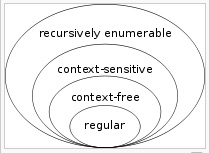
\includegraphics[height=30mm,width=35mm]{images/chomsky-hierarchy}
\end{center}


\end{frame}

\begin{frame}[fragile]{Grammars}

{\bf Observation:} The most convenient language class for programming language specification are the context-free
languages -- they are decidable -- pushdown automata can be efficiently implemented in order to prove language membership.
\end{frame}

\begin{frame}[fragile]{Grammars}

\scriptsize
{\bf Example:} A simple imperative language.  We define grammar $G=(\Gamma,\rightarrow,\gamma)$ as follows:
\begin{itemize}
\item $\Gamma = T \cup N$ where
{\tiny
\[
T =\{\term{0},\ldots,\term{9},\term{a},\ldots,\term{z},\term{true},\term{false},\term{skip},
\term{if},\term{then},\term{else},\term{while},\term{do},\term{end}+,-,*,=,\le,!,\&\&,||,:=,;,(,)\}
\]
}
and
{\tiny
\[
N = \{A,B,C,D,L,V\}.
\]
}
\item The rule set $\rightarrow$ is defined by,
{\tiny
\[
\begin{array}{rcl}
\nonterm{A} &\rightarrow& D \orbar V \orbar \nonterm{A} +\nonterm{A} \orbar \nonterm{A} - \nonterm{A} \orbar 
	\nonterm{A} * \nonterm{A}\orbar ( \nonterm{A} )\\

\nonterm{B} &\rightarrow& \mbox{\bf true} \orbar \mbox{\bf false} \orbar \nonterm{A} = \nonterm{A} \orbar
	\nonterm{A} \le \nonterm{A} \orbar ! \nonterm{B} \orbar \nonterm{B} \&\& \nonterm{B} \orbar 
	\nonterm{B} || \nonterm{B} \orbar (\nonterm{B})\\

\nonterm{C} &\rightarrow& \mbox{\bf skip} \orbar \nonterm{V} := \nonterm{A} \orbar\nonterm{C}\; ; \nonterm{C} \orbar
	\mbox{\bf if} \; \nonterm{B}\; \mbox{\bf then}\;\nonterm{C}\; \mbox{\bf else}\; \nonterm{C} \; \term{end}\orbar
	\mbox{\bf while}\; \nonterm{B}\; \mbox{\bf  do}\; \nonterm{C}\; \term{end}\\

\nonterm{D} &\rightarrow& \nonterm{L} \orbar - \nonterm{L}\\

\nonterm{L} &\rightarrow& \term{0}\, \nonterm{L} \orbar \ldots \orbar  \term{9} \,\nonterm{L} \orbar \term{0} \orbar \ldots\orbar\term{9}\\

\nonterm{V} &\rightarrow& \term{a}\,\nonterm{V} \orbar \ldots\orbar \term{z}\,\nonterm{V} \orbar \term{a} \orbar \ldots \term{z}
\end{array}
\]
}
\item $\gamma =\nonterm{C}$.
\end{itemize}

Observe that this is a context-free grammar!
\end{frame}

\begin{frame}{Grammars}
Here are some elements in $L(G)$,
\[
\begin{array}{l}
x := 1 ; y := x\\ 
v := 1; \ifstmt{v \le 0}{v := (-1)*v}{\term{skip}}\\
n := 5 ; f := 1 ; \whilestmt{2 \le n}{f := n*f ; n := n - 1}
\end{array}
\]
{\bf Exercise:} Prove that they belong to $L(G)$.

\end{frame}

\begin{frame}{Grammars}

HW\#1 -- see website

\end{frame}



\end{document}
